% !TeX spellcheck = en_US
\addscenariosection[subsection]{1}{Inferno Campaign $-$ Dungeons and Devils}{2. Steadwick's Fall}{\images/firewall.png}

\begin{multicols*}{2}

\textbf{Author:} Tm335

\textbf{Source:} \href{https://discord.com/channels/740870068178649108/1246353361456861276/1246353361456861276}{Archon Studios Discord}

\textit{Catherine Ironfist has enlisted aid from Bracada and AvLee.
She knows we are close to Steadwick.
We must occupy Steadwick before she arrives.
Once we own Erathia's capitol, not even Catherine Ironfist will wrench it from our hands.}

\subsection*{\MakeUppercase{Scenario Length}}

This Scenario plays out over 16 Rounds.

\subsection*{\MakeUppercase{Player Setup}}

\textbf{Faction:} Inferno

\textbf{Faction Hero:} Choose any

\textbf{Starting Resources:} 15 \svg{gold}, 1 \svg{building_materials}, 1 \svg{valuables}

\textbf{Starting Income:} 10 \svg{gold}, 2 \svg{building_materials}, 0 \svg{valuables}

\textbf{Starting Units:}

\begin{itemize}
  \item A Few Troglodytes
  \item A Few Evil Eyes
  \item A Pack of Familiars
\end{itemize}

\textbf{Town Buildings:} \svgunit{bronze} Dwelling, \svgunit{silver} Dwelling

\textbf{Bonus:} Choose one of the following options:
\begin{itemize}
  \item Add a Pack of Harpies to your hand.
  \item Add a Pack of Magogs to your hand.
  \item Add an Ammo Cart to your hand.
  \item Search (4) the Spell Deck.
\end{itemize}

\subsection*{\MakeUppercase{AI Hero Setup}}

\textbf{Faction:} Castle

\textbf{Enemies:} General Kendal, Charging Heroes

\textbf{General Kendal's Army:} A Pack of Archangels, a Pack of Champions, a Pack of Zealots, a Pack of Crusaders, a Pack of Griffins, a Balista War Machine

\textbf{General Kendal's Deck:} 5 × Might Card, 1 × Magic Card, 3 × Skill Card

\textbf{General Kendal's Spell Deck:} 2 × Haste Spell Card

\textbf{General Kendal's Skill:} Artillery Ability Card\footnote{For General Kendal, the Artilery Ability Card always resolves the Expert effect and the Ballista War Machine Activates every time the Artillery Ability Card is drawn, as well as at the beginning of a Combat Round.}

\textbf{Charging Heroes' Factions:} Rampart, Tower, Castle

\textbf{Charging Heroes' Armies:} Neutral Army is one Level higher than your Hero Level (Max Level VI)\footnote{See page 35, ``Field Difficulty Level Table'' in the Core Rulebook, for further details on the number of Neutral Units you have to draw for this Neutral Army.}.

\textbf{Charging Heroes' Deck:} 2 × Might Card, 2 × Magic Card

\textbf{Charging Heroes' Spell Deck:} 2 × Slow Spell Card\footnote{All the Charging Heroes' Enemies use the same AI and Spell Decks. Reset them after every Combat.}.

\subsection*{\MakeUppercase{Map Setup}}

Take the following Map Tiles and set them up as shown in the Scenario map layout:

\textbf{2 × Starting (I) Map Tile}
\begin{itemize}
  \item 1 × Inferno (S6)
  \item 1 × Castle (S3)
\end{itemize}

\textbf{3 × Far (II--III) Map Tile}
\begin{itemize}
  \item 1 × Castle (F3)
  \item 1 × Rampart (F10)
  \item 1 × Dungeon (F2)
  \item 1 × Tower (\#F1)
  \item 1 × Rampart (choose from: F11, F12)
  \item 1 × Necropolis (choose from: F4, \#F6, F7)
\end{itemize}

\textbf{2 × Near (IV--V) Map Tile}
\begin{itemize}
  \item 2 × Castle (N3, choose from: \#N3, N6)
  \item 1 × Rampart (N8)
  \item 1 × Necropolis (N4)
\end{itemize}

\subsection*{\MakeUppercase{Heroes Placement}}

The Enemy Hero General Kendal is represented by one Castle Faction Hero model and appears on the center Field of the S3 Starting Map Tile.

The Castle Charging Hero is represented by one Castle Faction Hero model and appears on (and owns) the Settlement of the F3 Map Tile.

The Rampart Charging Hero is represented by one Rampart Faction Hero model and appears on (and owns) the Settlement of the F10 Map Tile.

The Tower Charging Hero is represented by one Tower Faction Hero model and appears on (and owns) the Settlement of the \#F1 Map Tile.

Place your Main Hero on the center Field of the Inferno Starting S6 Map Tile.

Place your Secondary Hero, represented by one Dungeon Faction Hero model of your choice, on the Settlement of the F2 Map Tile. This Settlement produces no resources.

\subsection*{\MakeUppercase{Victory Conditions}}

Defeat all 3 Enemy Controlled Settlements (F3, F10, \#F1), and capture Steadwick (S3) before
Queen Catherine Ironfist arrives at the end of the Round 16.

\subsection*{\MakeUppercase{Defeat Conditions}}

You lose one Combat encounter with your Main Hero (Surrendering costs 10 \svg{gold}, and does not count as a defeat).

You lose your Faction Town on the S6 Map Tile.

You run out of time -- you have time till the end of the Round 16.

\subsection*{\MakeUppercase{Timed Events}}

\textbf{\nth{1} Round:}
\begin{itemize}
  \item Read: ``You are to be congratulated on your progress so far.
    You have laid waste to Eastern Erathia, and are now within striking distance of the Erathian
    capital of Steadwick. You must capture the capital quickly!''
\end{itemize}

\textbf{\nth{2} Round:}
\begin{itemize}
  \item Read: ``Not only have Bracada and AvLee sent reinforcements, but we have received news that
    Queen Catherine Ironfist is marching a sizeable army from the south. We must control the capital and its
    garrisons before she arrives.

    You have just received a report on the progress of Queen Catherine.
    Forces from Nighon and Eeofol are attempting to delay her march to Steadwick,
    but doubt that they can delay her more than two or three months.''
\end{itemize}

\textbf{\nth{5} Round:}
\begin{itemize}
  \item Read: ``You receive a report from the south. Queen Catherine's forces have been sufficiently delayed,
    allowing you at least two months more to reach the capitol, but our own forces have suffered significant
    losses. Do not let their sacrifice go to waste.''
\end{itemize}

\textbf{\nth{10} Round:}
\begin{itemize}
  \item For any Enemy Settlements (F3, F10, \#F1) that have not been defeated, an additional Enemy
    Charging Hero of that Faction appears on each Settlement.
\end{itemize}

\textbf{\nth{11} Round:}
\begin{itemize}
  \item Read: ``You receive a report from the south. Our forces continue to throw themselves in the path of
    Queen Catherine's armies, yet she continues to march northward. You have, at most, three or four weeks
    before she can reach the capital.''
\end{itemize}

\textbf{\nth{13} Round:}
\begin{itemize}
  \item Warning: ``Queen Catherine's march continues -- her forces are just two weeks away. If you do not hurry,
    we will not have time to secure the capital before her arrival.''
\end{itemize}

\textbf{\nth{15} Round:}
\begin{itemize}
  \item Warning: ``Your scouts report sighting Queen Catherine's army seven days to the southwest. If she
    reaches the capitol before you, all is lost.''
\end{itemize}

\textbf{\nth{16} Round:}
\begin{itemize}
  \item If Steadwick has not been taken, read: ``This morning, a massive army lead by Queen Catherine
    Ironfist arrived at the Erathian capitol of Steadwick. We have no choice but to retreat our forces.
    You have failed us... miserably.''
\end{itemize}

\textbf{When you complete the Scenario:}
\begin{itemize}
  \item Read: ``Congratulations! You captured Steadwick and are victorious!''
\end{itemize}

\subsection*{\MakeUppercase{Additional Rules}}

During this ``Inferno'' Campaign Scenario, the following rules apply:

\begin{itemize}
    \item The General Kendal Hero does not move and only waits in their Town. They start with Walls, a Gate,
      and an Arrow Tower on their side of the Combat Board.
    \item The difficulty Level of every Combat encounter on the map increases by one till the end of the Scenario
      (see page 35, ``Field Difficulty Level Table'' in the Core Rulebook).
    \item The Enemy Charging Heroes have only 2 Movement Points, instead of 3. They ignore everything else
      (including Mines and Settlements if possible) and go straight for the player's Faction Town (on Map Tile S6).
      They do not pursue the player directly, but if they happen to be on the same Map Tile, they will
      attack the player's Main Hero (not Secondary).
    \item The Enemy Charging Heroes move after the player's Turn ends.
    \item The borders on the Castle Starting Map Tile S3 cannot be crossed by any means until
      all Enemy Settlements (F3, F10, \#F1) have been defeated.
    \item Defeating Enemy Charging Heroes provides 2 \svg{valuables}.
    \item Obelisks give you 1 \svg{valuables} and function as a ``Castle
      Gate'' location (only if you have the ``Castle Gate'' built in your Town).
\end{itemize}

% \vspace*{\fill}
\begin{center}
  \framedimage[\columnwidth]{\art/demon.jpg}
\end{center}
% \vspace*{\fill}

\end{multicols*}

\begin{tikzpicture}[remember picture, overlay]
  \node(bg)[anchor=center, yshift=37em, opacity=0.17] at (current page.south) {
    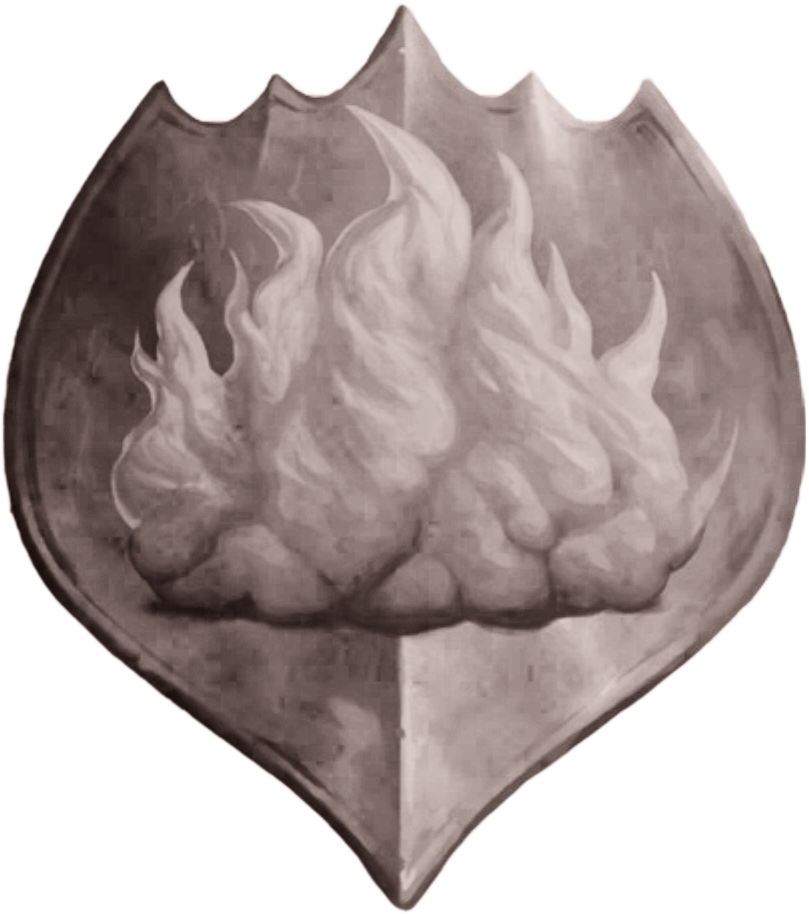
\includegraphics[width=0.85\paperwidth, keepaspectratio]{\art/fire_shield.png}
  };
  \node(map)[anchor=center] at (current page.center) {
    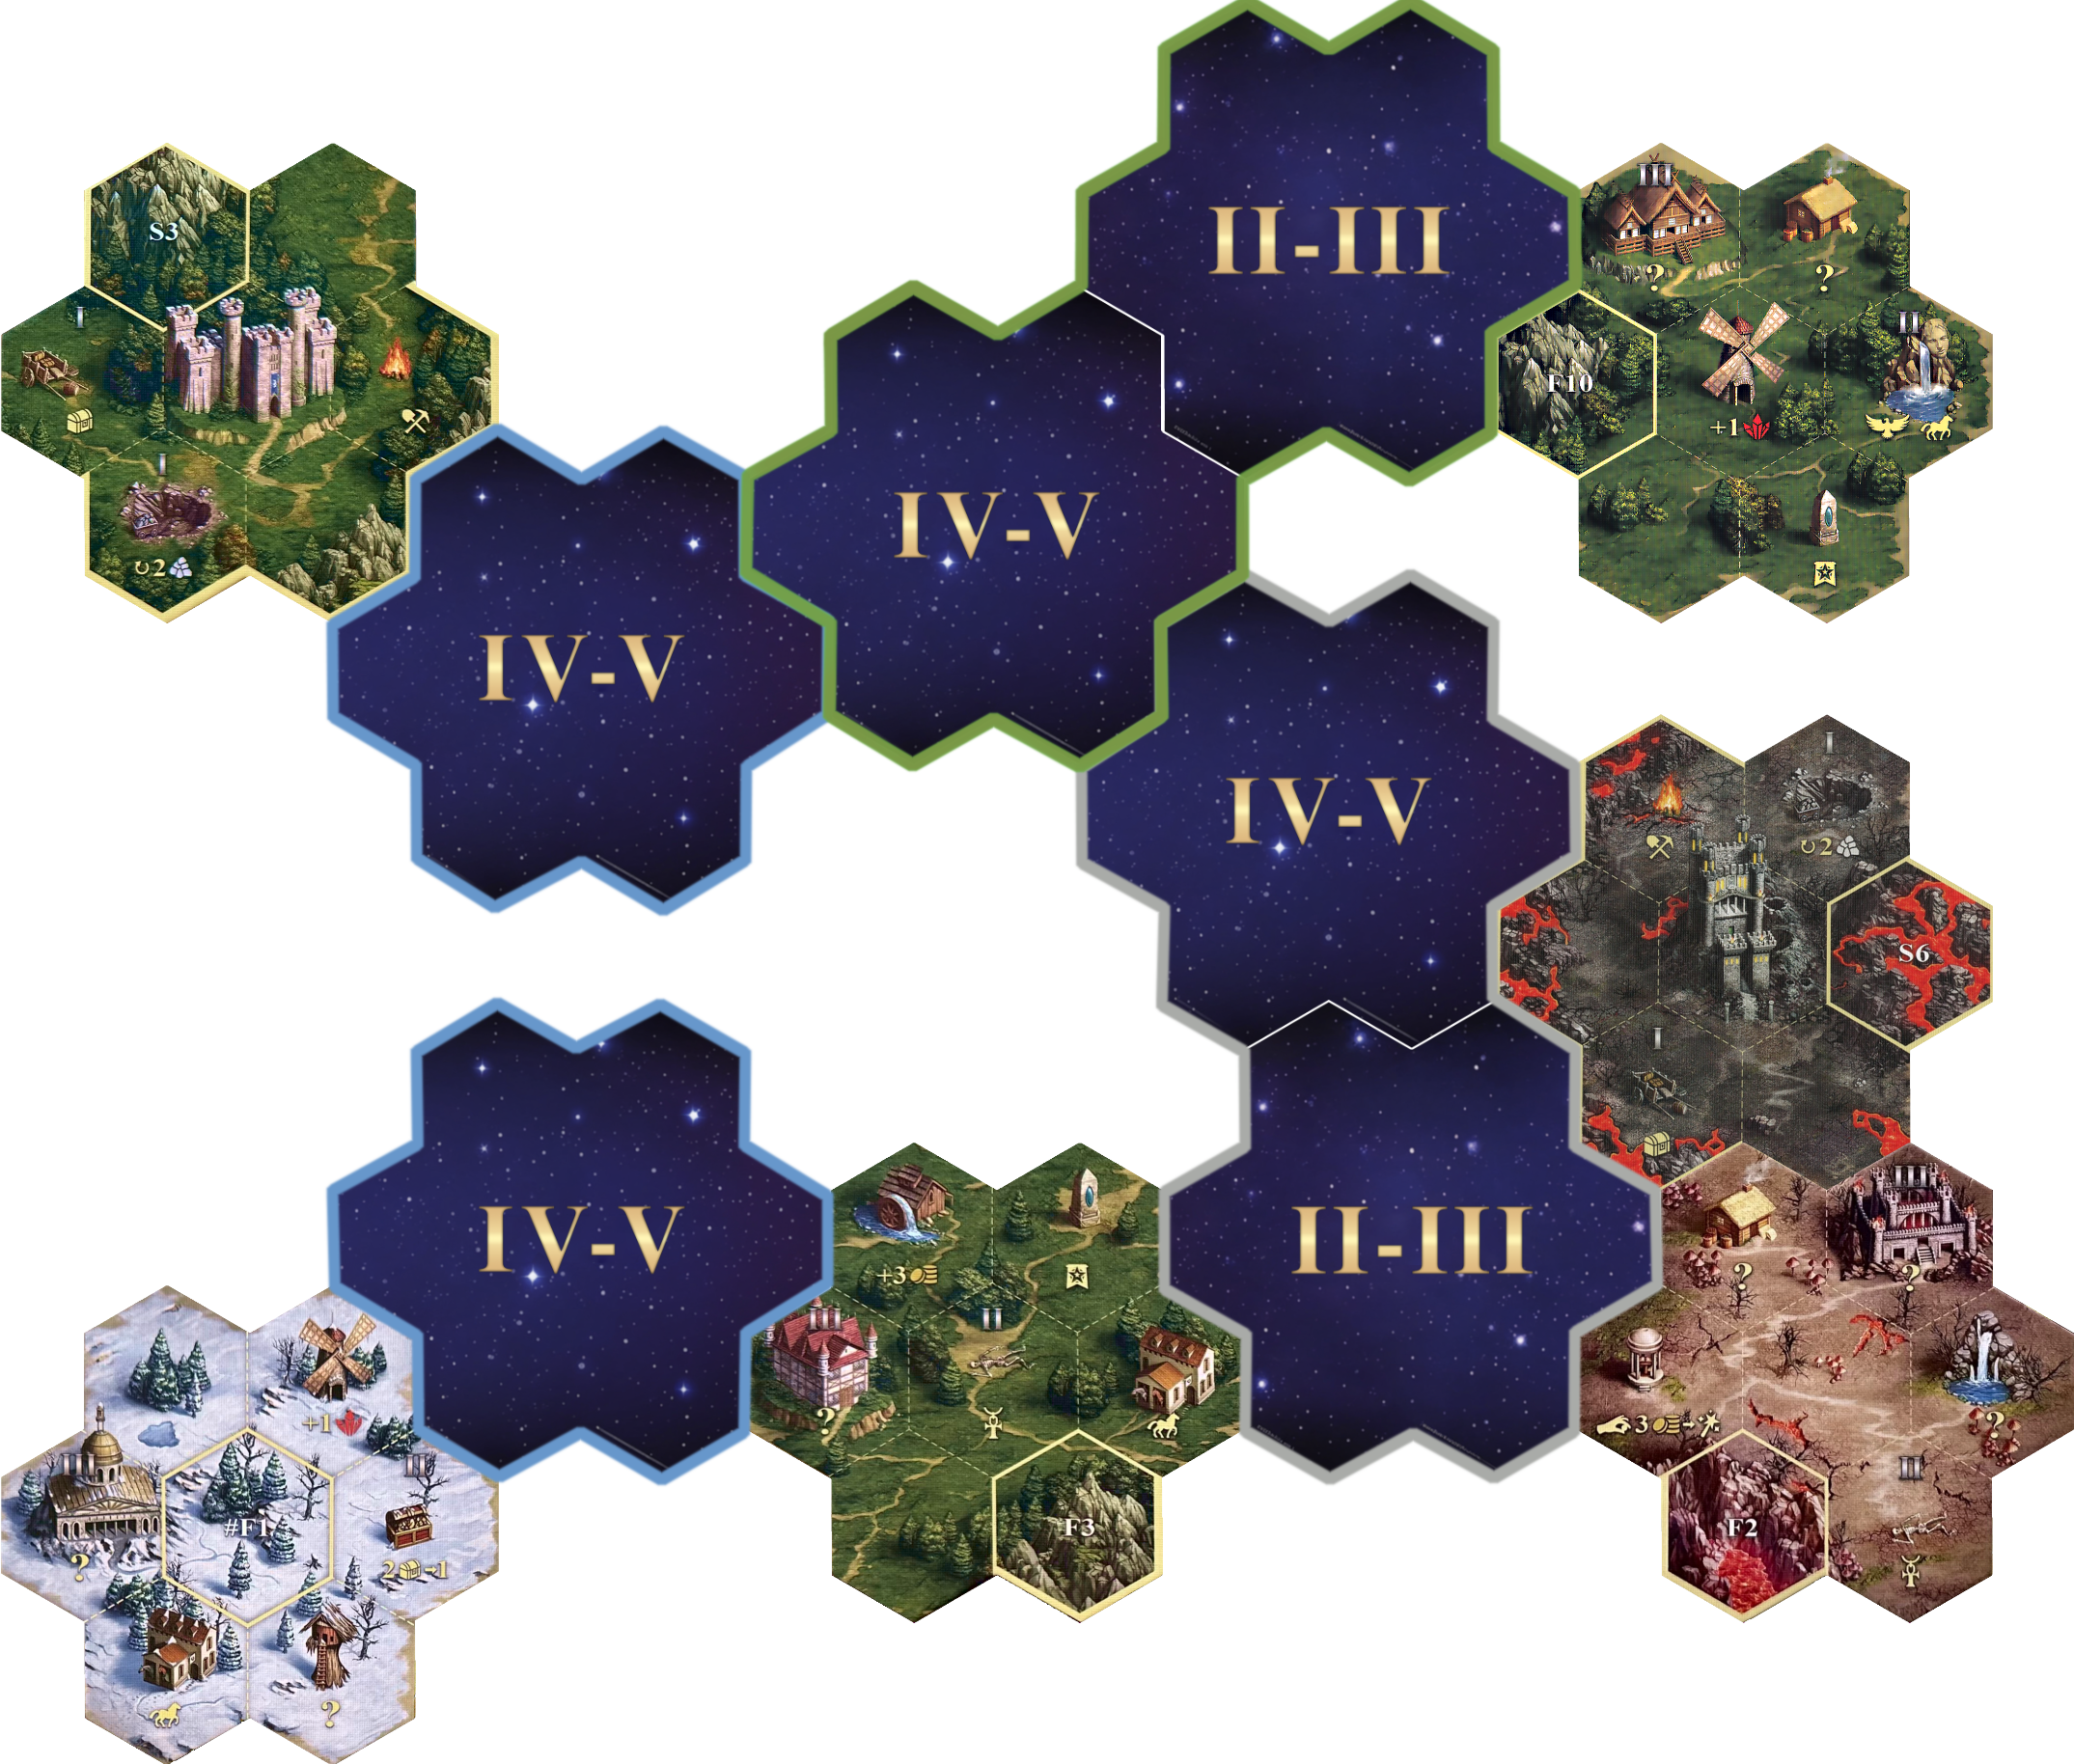
\includegraphics[width=\textwidth]{\maps/inferno_steadwicks_fall.png}
  };

  \node at (3, -11.5) {\large{{\textbf{\textcolor{darkcandyapplered}{N3}}}}};
  \node at (4.4, -18.6) {\large{{\textbf{\textcolor{darkcandyapplered}{\#F1}}}}};
  \node at (15, -5.2) {\large{{\textbf{\textcolor{darkcandyapplered}{F10}}}}};
  \node at (17.3, -11.5) {\large{{\textbf{\textcolor{darkcandyapplered}{S6}}}}};
  \node at (8.8, -18.8) {\large{{\textbf{\textcolor{darkcandyapplered}{F3}}}}};
  \node at (15.9, -18.8) {\large{{\textbf{\textcolor{darkcandyapplered}{F2}}}}};
  \node at (2, -4.5) {\large{{\textbf{\textcolor{darkcandyapplered}{Steadwick}}}}};
  \node at (2, -5.2) {\large{{\textbf{\textcolor{darkcandyapplered}{S3}}}}};
  \node at (7.5, -5.4) {\large{{\textbf{\textcolor{darkcandyapplered}{Rampart}}}}};
  \node at (7.5, -6.1) {\large{{\textbf{\textcolor{darkcandyapplered}{Map Tiles}}}}};
  \node at (12.4, -17.8) {\large{{\textbf{\textcolor{darkcandyapplered}{Necropolis}}}}};
  \node at (12.4, -18.5) {\large{{\textbf{\textcolor{darkcandyapplered}{Map Tiles}}}}};
  \node at (2, -12.3) {\large{{\textbf{\textcolor{darkcandyapplered}{Castle}}}}};
  \node at (2, -13) {\large{{\textbf{\textcolor{darkcandyapplered}{Map Tiles}}}}};
\end{tikzpicture}
